% unicodeは、hyperrefへの指定で、pdfのメタデータにあるタイトルの文字化けを防ぐ
% ptは細かい指定はできないらしい
% A cheat sheet
% https://www.cpt.univ-mrs.fr/~masson/latex/Beamer-appearance-cheat-sheet.pdf
\documentclass[unicode, 14pt, aspectratio=169]{beamer}
\usetheme{titech}
\addbibresource{main.bib}
\date{\today}
\title{一貫性と可用性によるシステムの分類}
\author{\texttt{ryotaro612}}
\newcommand\blfootnote[1]{%
  \begingroup
  \renewcommand\thefootnote{}\footnote{#1}%
  \addtocounter{footnote}{-1}%
  \endgroup
}
\begin{document}
\begin{frame}[noframenumbering, plain]
\titlepage
\end{frame}
\section{Jepsen}

\begin{frame}
  \frametitle{Jepsen: 分散システムのテストフレームワーク\supercite{jepsen}}
  {\large Jepsenはフォールトインジェクションに特化}
  \begin{itemize}
  \item Clojureのライブラリ
  \item テストケースは次のProtocol\supercite{clojure-protocols}の実装
    \begin{itemize}
    \item 分散システムのクライアント
    \item 起こしたい障害
    \item クライアントの操作と障害のスケジュール
    \item 実行結果の確認
    \end{itemize}
  \item Jepsenに実装の呼出、実行履歴の管理、再現を移譲
  \end{itemize}
\end{frame}
\begin{frame}
  \frametitle{Jepsenの認知度}
  {\large テストしたシステムの数は45\supercite{jepsen-analysis}}
  \begin{itemize}
  \item テスト対象の例
    \begin{itemize}
    \item etcd
    \item PostgresSQL
    \item MongoDB
    \item Elasticsearch
    \item Cassandra
    \end{itemize}
  \item テスト対象のetcdからJepsenへの言及もある\supercite{jepsen-etcd}
  \end{itemize}
\end{frame}
\begin{frame}
  \frametitle{テスト対象を評価するときの課題}
  {\large どの一貫性と可用性のペアなら実装できるのか}
  \begin{description}[font=\normalfont\underline]
  \item[CAP定理の問題]
  \begin{itemize}[leftmargin=0cm,topsep=0pt,before=\leavevmode\vspace{8pt}]
  \item CAP定理\supercite{cap}の一貫性は線形化可能性\supercite{linearizability} 
  \item 線形化可能性以外の一貫性のモデルは対象外
  \item トリレンマではない。一貫性と可用性のトレードオフ\supercite{cap-twelve-years-later}
    \begin{itemize}
    \item ネットワーク障害時の一貫性と可用性の優先度を問う
    \item 二者択一ではない。複数の候補がある
    \end{itemize}
  \item 複数の矛盾する可用性の定義\supercite{kleppmann}    
  \end{itemize}    
  \end{description}

\end{frame}
\section{一貫性と可用性のパターン}
\begin{frame}
  \frametitle{\normalsize{Highly Available Transactions Virtues and Limitations\supercite{high}}}
  {\large 一貫性と両立できる可用性のペアを半順序関係に整理}
  \begin{columns}
    \begin{column}{0.5\textwidth}
      \begin{itemize}
      \item {\small ネットワークの無期限の分断を前提}
      \item {\small ノードは一貫性を表現}
      \item {\small 無枠はhigh availability,\\青枠はSticky availability\footnote{意味は後述}}
      \item {\small 楕円は実現できないペア}        
      \item {\small Jepsenのサイトに一貫性の\\解説がある\supercite{jepsen-models}}
      \end{itemize}
    \end{column}    
    \begin{column}{0.5\textwidth}
      \begin{figure}
        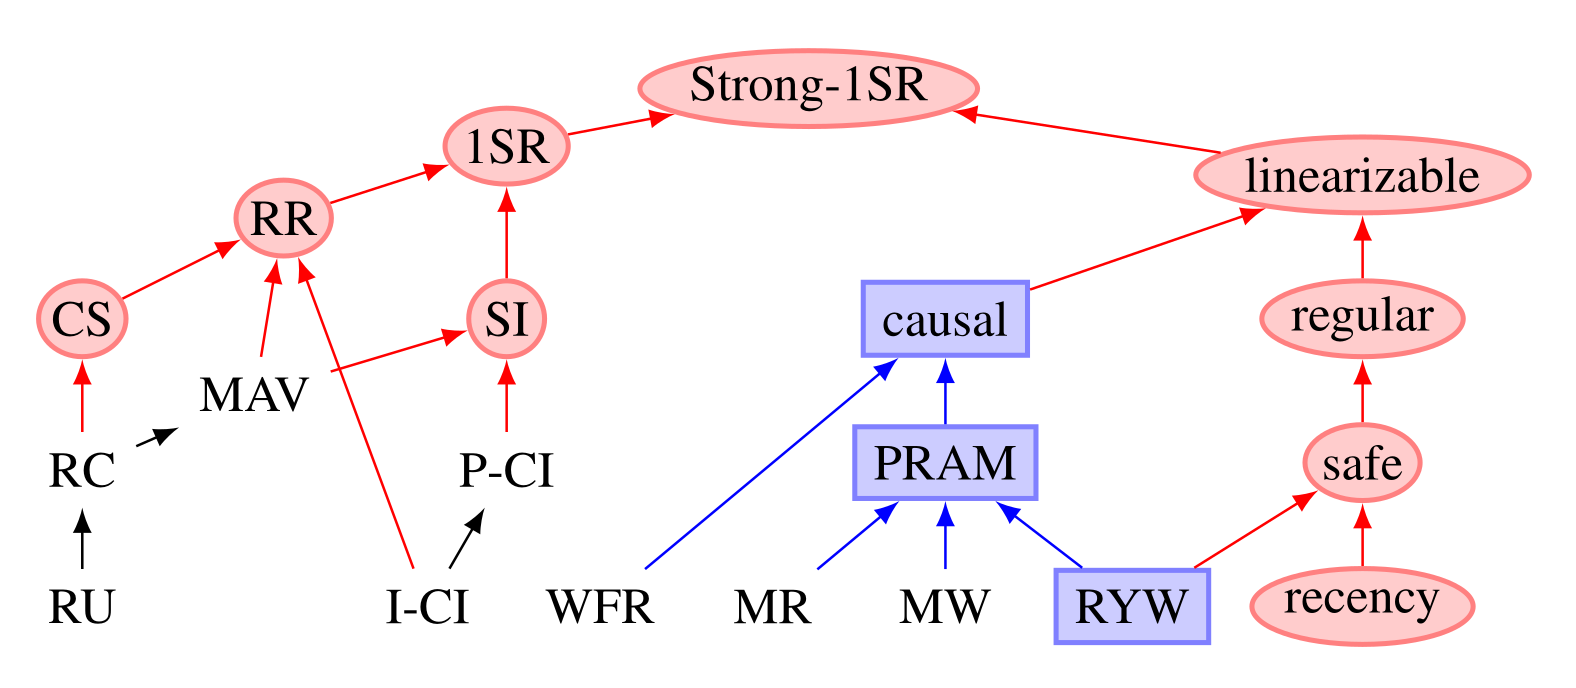
\includegraphics[width=1\textwidth]{images/hat.png}
        \caption{一貫性と可用性のペアの強さ\supercite{high}}
      \end{figure}
    \end{column} 
  \end{columns}
\end{frame}
\begin{frame}
  \frametitle{2つの可用性}
  {\large Sticky availabilityはHigh availablityの必要条件}
  \begin{description}
  \item[Sticky Availability]
    \begin{enumerate}[before=\leavevmode]
    \item クライアントによる過去の全操作を反映したレプリカがある
    \item クライアントが上のレプリカにトランザクションを実行する
    \item クライアントに応答が返る
    \end{enumerate}
  \item[High Availability]
    \begin{enumerate}[before=\leavevmode]
    \item 1つ以上の正常なサーバがある
    \item 上の1つにリクエストを送る
    \item クライアントに応答が返る
    \end{enumerate}
  \end{description}
  どちら可用性も応答にかかる時間は問わない
\end{frame}
\begin{frame}
  \frametitle{関係のあるペアの例}
  {\large WFRとcausalには強さに関係がある}
  \begin{description}
  \item[WFR (Writes Follow Reads, high availability)]
    \begin{enumerate}[before=\leavevmode]
    \item プロセスがトランザクション$T_1$をコミット
     \item 次に$T_2$をコミット
    \item 別のプロセスは$t_2$の結果を$t_1$の結果より前に参照できない
    \end{enumerate}
    % WFRをavailableなノードだけで実行するとcausalになる
  \item[causal (sticky availability)]
    \begin{enumerate}[before=\leavevmode]
      % ランチの誘い
    \item 因果関係のある操作の結果がすべてのプロセスから同じ順序で観測される
    \item 因果関係のない操作の観測順序は同一とは限らない
      \end{enumerate}
  % \item[linearizable] 読み書き操作がアトミックであるように観測でき、かつ、すべてのプロセスの実行を仮に直列化したときと同じ実行結果になる
  \end{description}
\end{frame}
\begin{frame}[allowframebreaks,t]
  \frametitle{参考資料}
  \printbibliography
  \nocite{*}
\end{frame}
\end{document}
